\documentclass[border=4pt,12pt]{standalone}
% House style for redrawn exam diagrams (diagram-v4: 0.4pt lines, filled -latex arrows, fine dashes; stipple and hatching drawn as real dots/lines (no PDF/SVG patterns, so they render in every browser and at any scale); transparent background). Every figure \input's this.
\usepackage{amsmath,amssymb}
\usepackage{txfonts}
\usepackage{pdfrender,xcolor}
% \halo{text}: label on shading. The shading stops just around each letter's outline (a thin knock-out that follows the
% glyphs, like the papers' typesetting), never a box. Owner: "I don't want a box around the text".
\newcommand{\halo}[1]{\leavevmode\rlap{\pdfrender{TextRenderingMode=2,LineWidth=2.2pt,LineJoinStyle=1,StrokeColor=white,FillColor=white}#1}#1}
\usepackage{tikz,pgfplots}
\pgfplotsset{compat=1.18}
\usetikzlibrary{arrows.meta,calc,angles,quotes,patterns,patterns.meta,intersections,positioning,decorations.markings,shapes.geometric}
% Stipple and hatching are drawn as actual dots / lines clipped to the region (path picture), NOT as pattern fills:
% SVG <pattern> fills vanish or blur when browsers scale the image, so the owner could not see the shading.
% Each dot is a 0.72pt square (keeps SVGs small; reads as a dot at print size). Dots sit on one global staggered grid, so neighbouring regions line up.
\makeatletter
\newdimen\ex@x \newdimen\ex@y \newdimen\ex@xa \newdimen\ex@ya \newdimen\ex@xb \newdimen\ex@yb \newcount\ex@row
\def\exam@stipplecolor{black!75}\def\exam@dotr{0.42pt}\def\exam@dotgap{2.5}
\def\ex@rowdots{\ifdim\ex@x<\ex@xb \pgfpathrectangle{\pgfqpoint{\dimexpr\ex@x-0.36pt\relax}{\dimexpr\ex@y-0.36pt\relax}}{\pgfqpoint{0.72pt}{0.72pt}}\advance\ex@x by \exam@dotgap pt\relax\expandafter\ex@rowdots\fi}
\def\exam@stipple{%
  \pgftransformreset% dots are sized in real points even inside scaled pictures
  \pgfpointanchor{path picture bounding box}{south west}\ex@xa=\pgf@x \ex@ya=\pgf@y
  \pgfpointanchor{path picture bounding box}{north east}\ex@xb=\pgf@x \ex@yb=\pgf@y
  \pgfsetfillcolor{\exam@stipplecolor}\pgfmathsetmacro\ex@h{\exam@dotgap/2}%
  \pgfmathtruncatemacro\ex@r{floor(\ex@ya/\ex@h)-1}\ex@row=\ex@r\relax
  \ex@y=\ex@r\dimexpr\ex@h pt\relax
  \loop\ifdim\ex@y<\ex@yb
    \pgfmathtruncatemacro\ex@c{floor(\ex@xa/\exam@dotgap)-1}\ex@x=\ex@c\dimexpr\exam@dotgap pt\relax
    \ifodd\ex@row \advance\ex@x by \ex@h pt\fi
    \ex@rowdots
    \advance\ex@y by \ex@h pt \advance\ex@row by 1
    \ifnum\numexpr\ex@row-(\ex@row/4)*4\relax=0 \pgfusepath{fill}\fi% flush every 4 rows: bounded TeX memory, few clip copies in the SVG
  \repeat\pgfusepath{fill}}
\newdimen\ex@d
\def\exam@hatch#1{% #1 = 1 for /, -1 for \ ; lines 45 degrees, 3pt apart
  \pgftransformreset
  \pgfpointanchor{path picture bounding box}{south west}\ex@xa=\pgf@x \ex@ya=\pgf@y
  \pgfpointanchor{path picture bounding box}{north east}\ex@xb=\pgf@x \ex@yb=\pgf@y
  \ex@d=\dimexpr\ex@yb-\ex@ya\relax \ex@x=\dimexpr\ex@xa-\ex@d\relax
  \loop\ifdim\ex@x<\ex@xb
    \ifnum#1>0 \pgfpathmoveto{\pgfqpoint{\ex@x}{\ex@ya}}\pgfpathlineto{\pgfqpoint{\dimexpr\ex@x+\ex@d\relax}{\ex@yb}}%
    \else \pgfpathmoveto{\pgfqpoint{\ex@x}{\ex@yb}}\pgfpathlineto{\pgfqpoint{\dimexpr\ex@x+\ex@d\relax}{\ex@ya}}\fi
    \advance\ex@x by 4.24pt
  \repeat
  \pgfsetlinewidth{0.4pt}\pgfsetstrokecolor{black}\pgfusepath{stroke}}
\def\examstipple{\exam@stipple}\def\examhatch{\exam@hatch}\def\examsetstipplecolor#1{\def\exam@stipplecolor{#1}}\def\examsetdotgap#1{\def\exam@dotgap{#1}}
\makeatother
% (legacy pattern kept for old files)
% staggered stipple like the NESA papers' dotted shading
\pgfdeclarepatternformonly{exam stipple}{\pgfpointorigin}{\pgfqpoint{2.2pt}{2.2pt}}{\pgfqpoint{2.2pt}{2.2pt}}{%
  \pgfpathcircle{\pgfqpoint{0.55pt}{0.55pt}}{0.42pt}\pgfpathcircle{\pgfqpoint{1.65pt}{1.65pt}}{0.42pt}\pgfusepath{fill}}
\tikzset{
  every picture/.style={line width=0.6pt, >={Latex[length=2mm,width=1.3mm]}},
  curve/.style={line width=0.6pt},
  open arrow/.style={-{Latex[length=2mm,width=1.3mm]}},  % owner: filled -latex heads everywhere, no open chevrons
  aux/.style={dash pattern=on 2pt off 1.5pt, line width=0.6pt},
  shade/.code={\def\exA{#1}\def\exB{none}\ifx\exA\exB\else\pgfkeysalso{fill=black!18}\fi},
  shade/.default=on,
  shade dots/.style={fill=none, path picture={\examstipple}},
  stipple color/.code={\examsetstipplecolor{#1}},
  stipple gap/.code={\examsetdotgap{#1}},
  shade dense dots/.style={fill=none, stipple gap=1.6, path picture={\examstipple}},
  shade hatch/.style={fill=none, path picture={\examhatch{1}}},
  shade hatch reverse/.style={fill=none, path picture={\examhatch{-1}}},
  shade solid/.style={fill=black},
  pt/.style={circle, fill, inner sep=1.1pt},
  open pt/.style={circle, draw, fill=white, inner sep=1.1pt},
}
\pgfplotsset{
  exam axes/.style={axis lines=middle, axis line style={->}, xlabel={$x$}, ylabel={$y$},
    xlabel style={anchor=west}, ylabel style={anchor=south}, tick label style={font=\small},
    every axis plot/.append style={line width=0.6pt, black}, samples=200, clip=false,
    enlargelimits=false, axis on top},
}

\begin{document}
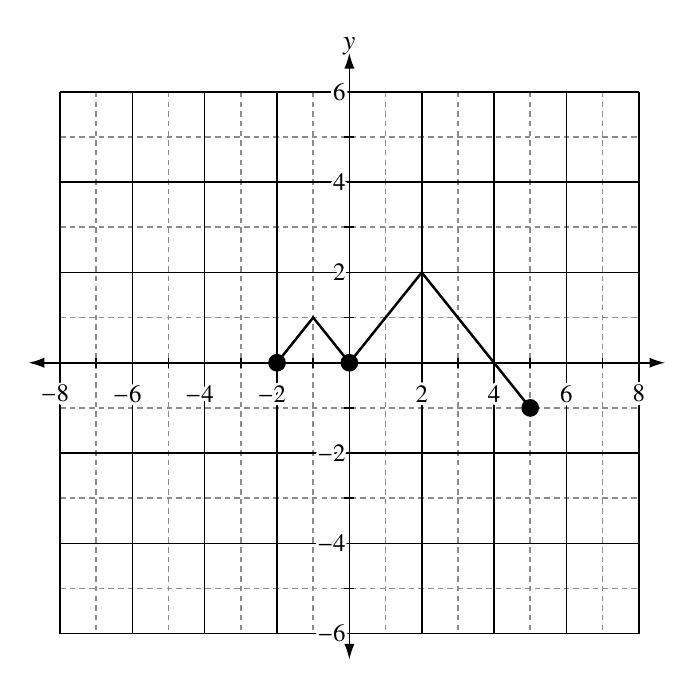
\begin{tikzpicture}[x=0.0127cm,y=-0.0127cm]
\draw[aux,black!45] (72.7,84.0) -- (72.7,626.0);
\draw[aux,black!45] (145.1,84.0) -- (145.1,626.0);
\draw[aux,black!45] (217.4,84.0) -- (217.4,626.0);
\draw[aux,black!45] (289.8,84.0) -- (289.8,626.0);
\draw[aux,black!45] (362.2,84.0) -- (362.2,626.0);
\draw[aux,black!45] (434.6,84.0) -- (434.6,626.0);
\draw[aux,black!45] (506.9,84.0) -- (506.9,626.0);
\draw[aux,black!45] (579.3,84.0) -- (579.3,626.0);
\draw[aux,black!45] (36.5,580.9) -- (615.5,580.9);
\draw[aux,black!45] (36.5,490.5) -- (615.5,490.5);
\draw[aux,black!45] (36.5,400.2) -- (615.5,400.2);
\draw[aux,black!45] (36.5,309.8) -- (615.5,309.8);
\draw[aux,black!45] (36.5,219.5) -- (615.5,219.5);
\draw[aux,black!45] (36.5,129.1) -- (615.5,129.1);
\draw (36.5,84.0) -- (36.5,626.0);
\draw (108.9,84.0) -- (108.9,626.0);
\draw (181.2,84.0) -- (181.2,626.0);
\draw (253.6,84.0) -- (253.6,626.0);
\draw (398.4,84.0) -- (398.4,626.0);
\draw (470.8,84.0) -- (470.8,626.0);
\draw (543.1,84.0) -- (543.1,626.0);
\draw (615.5,84.0) -- (615.5,626.0);
\draw (36.5,626.0) -- (615.5,626.0);
\draw (36.5,535.7) -- (615.5,535.7);
\draw (36.5,445.3) -- (615.5,445.3);
\draw (36.5,264.7) -- (615.5,264.7);
\draw (36.5,174.3) -- (615.5,174.3);
\draw (36.5,84.0) -- (615.5,84.0);
\draw[<->] (5,355) -- (642,355);
\draw[<->] (326,652) -- (326,45);
\draw (72.7,350) -- (72.7,360);
\draw (145.1,350) -- (145.1,360);
\draw (217.4,350) -- (217.4,360);
\draw (289.8,350) -- (289.8,360);
\draw (362.2,350) -- (362.2,360);
\draw (434.6,350) -- (434.6,360);
\draw (506.9,350) -- (506.9,360);
\draw (579.3,350) -- (579.3,360);
\draw (321,580.9) -- (331,580.9);
\draw (321,490.5) -- (331,490.5);
\draw (321,400.2) -- (331,400.2);
\draw (321,309.8) -- (331,309.8);
\draw (321,219.5) -- (331,219.5);
\draw (321,129.1) -- (331,129.1);
\node[font=\small,inner sep=0pt] at (31.5,386) {\halo{$-8$}};
\node[font=\small,inner sep=0pt] at (103.9,386) {\halo{$-6$}};
\node[font=\small,inner sep=0pt] at (176.2,386) {\halo{$-4$}};
\node[font=\small,inner sep=0pt] at (248.6,386) {\halo{$-2$}};
\node[font=\small,inner sep=0pt] at (398.4,386) {\halo{$2$}};
\node[font=\small,inner sep=0pt] at (470.8,386) {\halo{$4$}};
\node[font=\small,inner sep=0pt] at (543.1,386) {\halo{$6$}};
\node[font=\small,inner sep=0pt] at (615.5,386) {\halo{$8$}};
\node[font=\small,anchor=east,inner sep=0pt] at (323,626.0) {\halo{$-6$}};
\node[font=\small,anchor=east,inner sep=0pt] at (323,535.7) {\halo{$-4$}};
\node[font=\small,anchor=east,inner sep=0pt] at (323,445.3) {\halo{$-2$}};
\node[font=\small,anchor=east,inner sep=0pt] at (323,264.7) {\halo{$2$}};
\node[font=\small,anchor=east,inner sep=0pt] at (323,174.3) {\halo{$4$}};
\node[font=\small,anchor=east,inner sep=0pt] at (323,84.0) {\halo{$6$}};
\node[font=\normalsize] at (326, 38) {$y$};
\draw[line width=0.9pt] (253.6,355.0) -- (289.8,309.8) -- (326.0,355.0) -- (398.4,264.7) -- (506.9,400.2);
\fill (253.6,355.0) circle (3.2pt);
\fill (326.0,355.0) circle (3.2pt);
\fill (506.9,400.2) circle (3.2pt);
\end{tikzpicture}
\end{document}
